\newpage
\chapter{Plug flow reactor}

\section{Introduction}
The plug flow reactor model of Camflow simulates a one dimensional plug flow reactor with gas-phase chemistry. The model can handle a number of temperature conditions such as isothermal, non-isothermal, or user defined temperature profiles. 

\section{Fundamentals}
The plug flow reactor model solves the governing equations for continuity
\begin{equation}
 \frac{\rho u A_c}{dz} = 0,
\end{equation}
species continuity
\begin{equation}
 \rho u A_c\frac{dY_k}{dz} = W_kA_c\dot{\omega}_k \quad k=1\ldots K_g,
\end{equation}
energy equation
\begin{equation}
 \rho u A_c\frac{c_pdT}{dz} + \sum_{k=1}^{K_g} \dot{\omega}_kh_kW_kA_c = UA_s(T_w-T),
\end{equation}
and the equation of state
\begin{equation}
 p\bar{W}=\rho R T.
\end{equation}
In the above equations, $\rho$ is the density in kg/m$^3$, $u$ is the velocity in m/s, $A_c$ is the area of cross section in m$^2$, $Y_k$ is the mass fraction of the k\'th chemical species, $W_k$ is the molecular mass in kg/mol of the k\'th chemical species, $\dot{\omega}_k$ is the molar production rate in mol/m$^3$-s of the k\'th chemical species, $c_p$ the specific heat at constant pressure in J/mol-K, $T$ the temperature in K, $T_w$ is the temperature of the wall in K, $A_s$ is the surface area per unit volume, and $U$ is the over all heat transfer coefficient in J/m$^2$sK.

\section{Input file}
An example of ``camflow.xml'' is shown below
{\scriptsize{\begin{verbatim}
<?xml version="1.0" encoding="ISO-8859-1"?>
<camflow>
   <reactor model="plug">
    <diameter unit="m">0.015</diameter>
    <length unit="cm">5</length>
  </reactor>
  <op_condition>
     <step_ignite>10</step_ignite>
     <temperature>isothermal</temperature>
     <twall unit="K">1073</twall>
    <pressure unit="Pa">1e5</pressure>
  </op_condition>
  <inlet>
     <fuel>
       <velocity unit="m/s">0.1</velocity>
       <temperature unit="C">800</temperature>
       <!--flowrate unit="cgs">4.63e-3</flowrate-->
       <molefrac>
        <species name="NO2">0.1</species>
        <species name="N2">*</species>
       </molefrac>
     </fuel>
  </inlet>
  <solver mode="coupled" solver="cvode">
     <tols>
        <species>
           <aTol>1.e-06</aTol>
           <rTol>1.e-06</rTol>
        </species>
        <temperature>
           <aTol>1.e-03</aTol>
           <rTol>1.e-03</rTol>
        </temperature>
        <flow>
           <aTol>1.e-03</aTol>
           <rTol>1.e-03</rTol>
        </flow>
     </tols>
  </solver>
  <initialize>    
    <Tprofile unit_L="cm" unit_T="K">
      <position x="0.0">373.7</position>
      <position x="0.125">484.5</position>
      <position x="0.25">583.7</position>
      <position x="0.375">672.2</position>
      <position x="0.5">753.5</position>
      <position x="0.75">901.4</position>
      <position x="1.0">1027.0</position>
      <position x="1.25">1120.0</position>
      <position x="1.5">1184.0</position>
      <position x="2.0">1260.0</position>
      <position x="3.0">1348.0</position>
      <position x="6.0">1475</position>
      <position x="10.0">1524.0</position>
    </Tprofile>
 </initialize>
 <report species="mole">
 </report>
</camflow>

\end{verbatim}}

}

The input file follows xml specification with a number of child elements. Each child element is described in detail below.

\begin{itemize}
 \item \textbf{rector} : The reactor element specifies which reactor models is to be simulated and for a plug flow reactor camflow expects plug as the model attribute value. The reactor element also holds child element for specifying reactor diameter and the reactor length, and each child element is given with the unit attribute. The unit of the value specified can be in ``cm'', ``m'', or in ``in''ches. Appropriate attribute must be specified.

\item \textbf{op\_conditions} : The element op\_conditions describes the operating conditions for the plug flow reactor. This includes the specification of the pressure and the condition applied to the solution of energy equation. The reactor pressure may be specified in the units of ``Pa'', ``atm'', or ``bar''. The temperature unit can be either in ``K'' or in ``C''. The temperature element can take the values of ``isothermal'', ``adiabatic'', ``userdefined'', or ``nonisothermal''. In the case of isothermal calculation, the energy equation is not solved and the reactor is assumed to be at the same temperature as the incoming fuel. The user may also perform the integration for a pre-calculated or measured temperature profile. In this case the temperature child element must be assigned with the value ``userdefined'' and the user defined temperature profile cane specified (explained later). For adiabatic calculations, provide the temperature element with the value ``adiabatic''. Radiation heat losses from the reactor are completely neglected. For non-isothermal calculation it is mandatory to specify the reactor wall temperature. The heat transfer coefficient is calculated internally as a function of reactor position using the following correlation.
\begin{equation}
 Nu= \frac{hD}{k},
\end{equation}
where $Nu$ is the Nusselt number, $h$ the heat transfer coefficient, $D$ the diameter and $k$ the thermal conductivity. The Nusselt number is defined as
\begin{equation}
 Nu = 3.657+8.827\bigg(\frac{1000}{\mathrm{Gz}}\bigg)^{-0.545} \exp\bigg(\frac{-48.2}{\mathrm{Gz}}\bigg),
\end{equation}
and the Greatz number Gz is defined as
\begin{equation}
 \mathrm{Gz} = \frac{D Re Pr}{z}
\end{equation}
with D the diameter, $Re$ the Reynolds\'s number, $Pr$ the Prandtl number, and $z$ the axial position of the reactor. In this version, the overall heat transfer coefficient is replaced with the heat transfer coefficient calculated from Nusselt number. Strictly speaking the correlation presented above are valid only for a non-reacting multi-component gas mixture. However, the above correlations are used for reacting case as well due to the non-availability of better formulations.\\

\textbf{step\_ignite} is an option to evaluate the minimum temperature required to ignite the gas-mixture and is optional. However, if the user is not interested in the ignition temperature, this element should not be present in the inputfile. If its present then \textbf{step\_ignite} must specify the step for temperature increment, and the \textbf{temprature} specification must be ``adiabatic''. The ignition temperature calculated is not printed to the output file, rather only a screen output is generated.\\

\item \textbf{inlet} : The inlet element holds the information on reactants and the reactant temperature at axial position at z=0, and the flow rate or velocity at z=0; Either the velocity or the flow rate needs to be specified. The velocity may be specified in m/s or in cm/s, while the flow rate may be specified in ``cgs'' units or in ``si'' units. The temperature of the reactants must be specified using the temperature element with the appropriate units. The mass or mole fraction of the reactant species need to be specified within the element molefrac or massfrac. The sum of mass fractions or mole fraction of the reactant species must sum up to 1. Instead of specifying the mass/mole fractions of all species, the last species can be assigned with *. In this case the mole/mass fraction of the last species will be 1-sum of others.

\item \textbf{solver}: The solver element holds the solver control specifications. The attributes ``mode'' should always be specified as ``coupled'' for plug flow reactor simulation. The solver name is essentially provided to switch from one solver to another. However, the present version of Camflow uses only CVode as the numerical integrator, and therefore accepts only ``cvode'' as the solver name. The element ``tols'' hold the various tolarences that can be applied to the species, energy, and continuity equations. For species a relative tolarence of at least 10$^{-6}$ should be used. The user may need to adjust the tolarence values for the species in case of solution difficulties.

\item \textbf{initialize} The initialize element can be used to specify various initial conditions. However, for plug flow reactor model, the only initial property that can be specified is the user defined temperature profile. The temperature profile can be specified by using the ``Tprofile'' element with two attributes namely ``unit\_L'' for length unit and ``unit\_T'' for temperature unit. The length unit can be in ``cm'' or in ``m'', where as the temperature unit can be either in ``K'' or in ``C''. The actual temperature as a function of reactor position is specified with the child elements position with the attribute ``x'', which stands for the position with the reactor. If the length unit is specified as ``cm'' then ``x'' is the position from the reactor inlet in ``cm'', and the value for the position element is the temperature at position ``x''.

\item \textbf{report}: The desired output for the species composition must be specified in this element using the species attribute. ``mole'' or ``mass'' may be used as the attribute values, and correspondingly the output will be produced either in mole fraction or mass fractions.

\end{itemize}

\section{Executing the binary}
The plug reactor model of Camflow expects three input files namely, ``camflow.xml'', ``therm.dat'',  ``chem.inp''. For performing non-isothermal calculation an additional file ``tran.dat'' specifying the transport data of all chemical species present in the system need to be specified. All these files must be present in the working directory. Upon succesful execution the output file ``profile.dat'' containing the axial position (m), density (kg/m$^3$), velocity (m/s), massflow rate (kg/m$^2$s), residence time (1/s) temperature (K), and the species compositions in mass or mole fractions.

\section{Results}
The following figure shows the species profiles and temperature for Hydrogen oxidation reaction 
\begin{figure*}[h]
 \centering
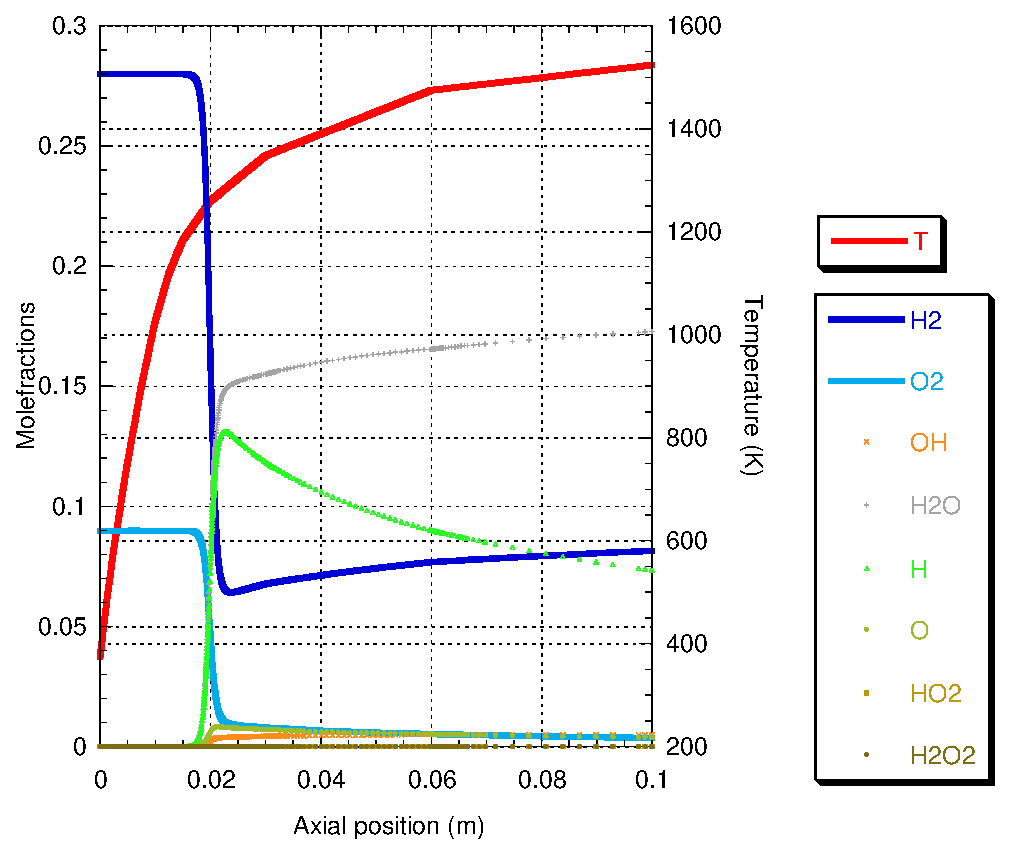
\includegraphics[scale=0.6]{plug_profile.eps}
\caption{Species profiles hydrogen oxidation with user defined temperature profile}
\end{figure*}

%===============================================================================================
%
%
%
%===============================================================================================

